%! Author = Saeid Yazdani
%! Date = 1/6/2024


%%%%%%%%%%%%%%%%%%%%%%%%%%%%%%%%%%%%%%%%%%%%%%%%%%%%%%%%%%%%%%%%%%%%%%%%%%%%%%%%


\section{Challenges in \acs{ATE} Environments}
\label{sec:ate-env}
%%%%%%%%%%%%%%%%%%%%%%%%%%%%%%%%%%%%%%%%%%%%%%%%%%%%%%%%%%%%%%%%%%%%%%%%%%%%%%%%

Tests are usually carried out either at \emph{wafer} stage or after
\emph{packaging} (also known as \emph{End Test} or \emph{Final Test}).

The goal of wafer testing, or \emph{Wafer Sort}, is to find all functional
bare dies from the wafer to sort out faulty dies before cutting
the wafer into individual chips.
This will reduce the cost of packaging and time for testing
non-functional packaged \ac{IC}.

In addition to various tests discussed in \autoref{sec:bist-vs-ate} (parametric, logic, 
analog, etc.), \emph{Burn-In} tests can also be carried out by an \ac{ATE} equipped 
with a thermal head, as shown in \autoref{fig:thermal-head-on-ate}. While such 
thermal heads are commonly used in laboratory or failure analysis setups, they can 
also be employed during testing to elevate the \ac{DUT} temperature and observe its 
behavior under stress, thereby simulating harsh environmental conditions in a 
controlled manner.

\begin{figure}[h]
    \centering
    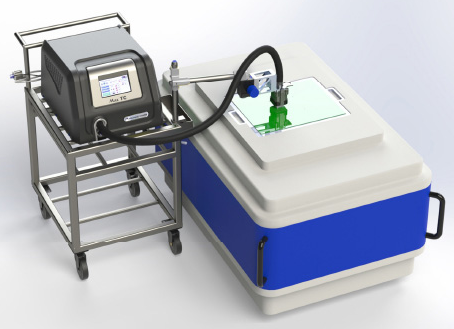
\includegraphics[scale=0.40]{figures/thermal-head-on-ate}
    \caption[Thermal Head over \ac{DUT}]{
        Thermal head positioned over a \ac{DUT} during \ac{ATE} testing, 
        controlled to reach a specified temperature setpoint.
        (\copyright M.D. Mechanical Devices)
    }
    \label{fig:thermal-head-on-ate}
\end{figure}

Test yield depends not only on the test strategy and algorithms but also on the 
quality of signals in the test equipment and on process control in fabrication 
(i.e., the uniformity and stability of device parameters across wafers). Test 
vectors and stimuli are affected by degrading effects such as noise, attenuation, 
distortion, and crosstalk. Optimized wiring is essential for fast and
reliable \ac{IC} testing.

The fact that multi-gigabit data rates and internal clocks above
\SI{1}{\giga\hertz} are becoming normal in modern \acp{IC} and their
\ac{I/O} cells, one of the key challenges for \acp{ATE} is delivering power and
data signals to the \ac{DUT} while maintaining the integrity of test signals
(rise and fall times, jitter, etc.) and exhibiting little to no
supply fluctuations (overshoot or undershoot, switching noise, etc.).

\autoref{fig:dut-in-native-vs-ate-env} illustrates an \ac{IC} in its native
environment and in a test environment.
When a chip sits on a \ac{PCB}, the distance between power regulators and
other circuit elements are usually very short and traces on the layout are
optimized to the best extent.
On the contrary, an \ac{ATE} must provide the test signals from a much greater
distance and the signals must go through a lot of interconnects to reach the
\ac{DUT}.

\begin{figure}[h]
    \centering
    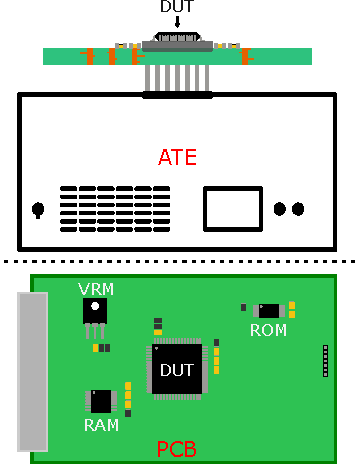
\includegraphics[scale=1.08]
    {figures/dut_environment_native_vs_test}
    \caption[\acs{DUT} in application and in tester]{A Comparison between
    the \ac{ATE} test environment (top) and native operation
    environment (bottom) for a given \ac{DUT}.
    Signal paths, power delivery and placement of support components are
    highly optimized in comparison to \ac{ATE} environment.}
    \label{fig:dut-in-native-vs-ate-env}
\end{figure}

Meanwhile, from an economic point of view, \acp{ATE} are required to be as
generic as possible to have the ability to test a broad range of devices
in terms of functionality and packaging \autocite{Pointl}, especially
considering that the initial investment and running maintenance costs
for some of the more advanced \ac{ATE} models can reach beyond millions of
dollars.
That is, designing an \ac{ATE} for test and qualification of a single product
is most likely not a viable option.

%%%%%%%%%%%%%%%%%%%%%%%%%%%%%%%%%%%%%%%%%%%%%%%%%%%%%%%%%%%%%%%%%%%%%%%%%%%%%%%%

\subsection{A Closer Look into \acs{ATE} Internals}
\label{subsec:ate-anatomy}
%%%%%%%%%%%%%%%%%%%%%%%%%%%%%%%%%%%%%%%%%%%%%%%%%%%%%%%%%%%%%%%%%%%%%%%%%%%%%%%%

To be general-purpose and flexible, \ac{ATE} platforms are usually built with a
fixed base unit or main frame that exposes test pins on a test-head for
interfacing with \ac{DUT}-specific \emph{load boards}.
This configuration will allow an \ac{ATE} to interface with multiple \acs{DUT}
types through the use of a \acp{DIB} or \emph{load boards}\footnote{Also commonly
known as \enquote{Test Fixture} or \enquote{Daughter Card}.}.
\autoref{fig:advantest-93k} shows a modern \ac{ATE} system and its main parts:

\begin{itemize}[topsep=8pt,itemsep=4pt,partopsep=4pt, parsep=4pt]

    \item \textbf{\emph{Base Unit}:}
    The base unit in most \ac{ATE} platforms is built around a modular concept
    where it contains a core management unit designated to handle internal power
    supply and other test-specific modules (digital, analog, \ac{RF}, etc.).
    The core management unit is what the test engineers can connect to through
    test software and coordinate test procedures as it handles the
    communication by dispatching commands to and receiving
    output from other modules.

    \item \textbf{\emph{Test Head} or {Mother Board}:}
    The test head is where the signals coming from \ac{ATE} modules and power
    supplies are exposed to the outside world.
    \paragraph{}{Test heads are an assembly of waveguides on a load board,
        pogo-pins between test head and load board, between load board and
        \ac{DUT} socket, and semi-rigid coaxial wiring for \ac{RF}.}

    \item \textbf{\emph{Support Unit}:}
    \acp{ATE} are complex systems and require a stable main power source and
    cooling solutions to keep the entire system at a constant temperature
    The laboratory or test floor needs to provide all necessary power
    and cooling for the \ac{ATE}.

\end{itemize}

\begin{figure}[htbp]
    \centering
    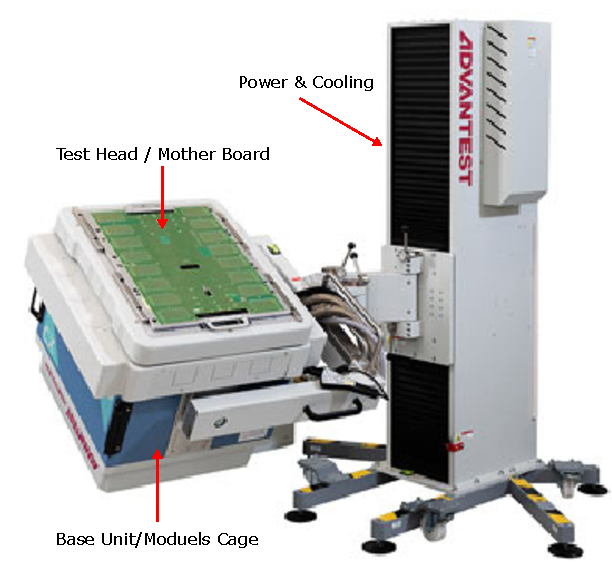
\includegraphics[width=0.86\linewidth,height=0.50\textheight,keepaspectratio]
    {figures/ate_structure_advantes_93k}
    \caption[A Modern \acs{ATE} setup]{A Modern \ac{ATE}
    platform consists of a base unit exposing the test head
    accompanied by integrated power and
    liquid cooling tower (\copyright Advantest Corp.).}
    \label{fig:advantest-93k}
\end{figure}

\acp{ATE} are complex systems and, as a penalty for
being built modular and generic, their wiring scheme
consists of several levels of interconnects and wires.
\autoref{fig:ate-internal-wiring-scheme} shows internal diagrams of a typical
\ac{ATE} setup.

The first level of wiring and interconnects exists within the main unit, where
different modules are connected to the main control unit over a system bus.
The second layer of wiring connects each individual test module to the
test head.

At the top, a load board or probe card sits on top of the test head and
finally, the \ac{DUT} resides in a socket.
Signal and power paths between \ac{ATE} and \ac{DUT} form a complete loop.

Every interconnect in the path worsens
signal integrity and power delivery.
Therefore, the entire test setup should provide adequate bandwidth for
interfacing with a \ac{DUT}.
The bandwidth requirement for proper delivery and capture of test signals is
usually expected to be three times the \ac{DUT} clock rise or fall time
as an industry-accepted rule of thumb \autocite{Johnson}.

\begin{figure}[t!]
    \centering
    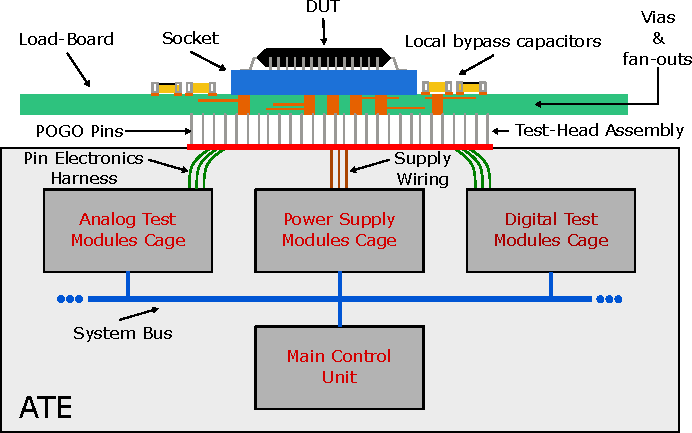
\includegraphics[width=0.82\textwidth]
    {figures/close_look_ate_dut_wiring}
    \caption[Internal wiring scheme of an \acs{ATE}]{A Closer look into the
    wiring scheme between an \ac{ATE} and a \ac{DUT}.}
    \label{fig:ate-internal-wiring-scheme}
\end{figure}

%%%%%%%%%%%%%%%%%%%%%%%%%%%%%%%%%%%%%%%%%%%%%%%%%%%%%%%%%%%%%%%%%%%%%%%%%%%%%%%%

\subsection{Challenges with Load Boards}
\label{subsec:loadboard-challenges}
%%%%%%%%%%%%%%%%%%%%%%%%%%%%%%%%%%%%%%%%%%%%%%%%%%%%%%%%%%%%%%%%%%%%%%%%%%%%%%%%

Connecting \acp{DUT} to an \ac{ATE} is based on
custom designed \emph{load boards}, if \acp{DUT} are already packaged, or
a \emph{probe card} in case of wafer-level testing.

An ideal load board should behave as if it were non-existent, meaning it should
not negatively affect the quality of test signals and power delivery.
In reality, each trace and via introduces parasitic properties in the form
of extra resistance, capacitance, and inductance in the signal path
that reduces signal quality.

Therefore, it is vital that during the design and layout of load boards, wries
should be treated like transmission lines
with constant impedance to minimize signal
degradation caused by reflections, distortions, and other parasitic effects.

Given the large size of \ac{ATE} test heads, trace lengths on a load
board might exceed \SI{50}{\centi\meter} in length in order to
bring signals from the edges of the test head to the \ac{DUT} site, which is
usually placed at the center of a load board.

The designer must consider
trace width and thickness, positioning of the traces in the
layer stack, and distribution of power planes.
Correct selection of substrate and dielectric material (\autoref{fig:dielectric-intel}) provides a uniform layer
thickness as material must tolerate production-induced stress such as
plating and soldering \autocite{dielectric}.

As the load boards for high pin-count \acp{DUT} come in a double-digit layer
count, the use of vias for transferring signals between layers is inevitable.
Special care is necessary when choosing via types
based on their manufacturability and electrical properties.

%%%%%%%%%%%%%%%%%%%%%%%%%%%%%%%%%%%%%%%%%%%%%%%%%%%%%%%%%%%%%%%%%%%%%%%%%%%%%%%%

\subsection{Challenges with \acs{ATE} Power Supplies}
\label{subsec:powersupply-challenges-in-ate}
%%%%%%%%%%%%%%%%%%%%%%%%%%%%%%%%%%%%%%%%%%%%%%%%%%%%%%%%%%%%%%%%%%%%%%%%%%%%%%%%

As stated in \autoref{sec:ch1-introduction}, the trend in \ac{VLSI}
over the last decades has been lowering the feature size in order to pack more
transistors into devices.
With lower feature size the thickness of the gate oxide in transistors also
decreases and hence the ability to withstand high electric fields without
breaking down is reduced.
Other issues like \emph{Short-Channel Effects} and
\emph{Leakage Currents} call for reduced core voltages.
Therefore the core voltage ratings for modern integrated circuits
are in a downtrend, as shown in \autoref{fig:featsize-vs-corevolt}.

\begin{figure}[htbp]
    \centering
    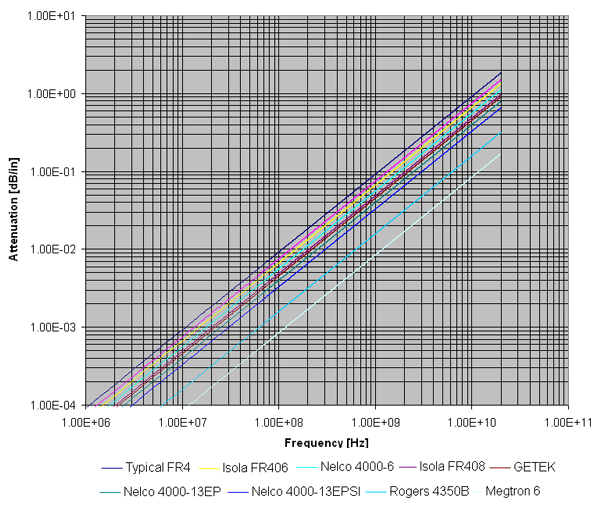
\includegraphics[width=0.64\linewidth,height=0.38\textheight,keepaspectratio]
    {figures/dielectric-chart-intel}
    \caption[Dielectric Absorption due to Loss Tangent]
    {
        Dielectric absorption due to \emph{Loss Tangent} or
        \emph{Dissipation Factor} ($D_f$) which is a
        measure for signal attenuation as the signal propagates through
        a transmission line.
        This attenuation is caused by electromagnetic wave absorption in
        the dielectric material in which the signal travels
        \autocite{intel-dielectronic}.
    }
    \label{fig:dielectric-intel}
    \vspace{-0.2\baselineskip}
\end{figure}

\begin{figure}[h!]
    \centering
    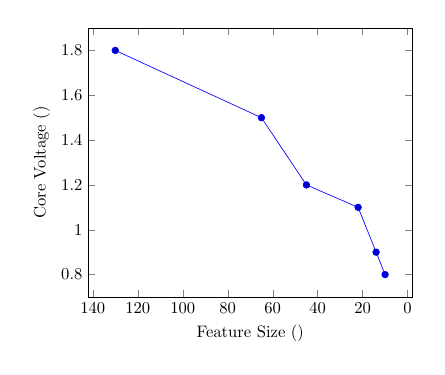
\begin{tikzpicture}[scale=0.60,transform shape]
        \begin{axis}
            [
            x dir=reverse,
            xlabel={Feature Size (\SI{}{\nano\meter})},
            ylabel={Core Voltage (\SI{}{\volt})},
            ]
            \addplot+ coordinates {
                (130,1.8)(65,1.5)(45,1.2)(22,1.1)(14,0.9)(10,0.8)
            };
        \end{axis}
    \end{tikzpicture}

    \caption[Feature Size v.s. Core Voltage]{
        The trend in core voltage of transistors is in a
        downtrend as the feature size shrinks.
    }
    \label{fig:featsize-vs-corevolt}
    \vspace{-0.8\baselineskip}
\end{figure}

At the same time, the increase in the number of transistors has resulted in
increased electrical current consumption of devices.
At low voltages and high currents, the power delivery can be negatively affected
by irregularities such as noise, overshoot, and undershoot.
Considering the long wiring and interconnects from the \ac{ATE} to the \ac{DUT},
delivering high currents at low voltages has made power integrity issues
a significant concern for the \acp{DUT} \autocite{Arabi}.

Recalling \autoref{fig:dut-in-native-vs-ate-env} and
\autoref{fig:ate-internal-wiring-scheme}, it is obvious that delivering such
low voltages and high currents is challenging when considering the
length and number of interconnects that the power lines need to travel to reach
the \ac{DUT}.

\enlargethispage{2\baselineskip}
Test yield can be negatively affected by variations of the power delivery
if a large current is required but cannot
be delivered promptly by \ac{ATE} power supply.
This can cause a \ac{DUT} \emph{false-negative} test result where otherwise a
functional \ac{DUT} is binned in the failing bucket.


Given that all the short-time support currents can only be supplied by
nearby capacitors, we need to understand the dynamics of support capacitors
in detail.

The total power analysis is based on the understanding of the \ac{RLC} behavior of
all DUT support capacitors: If there is a current request from the DUT we will
get a voltage drop of $\Delta V = L \frac{di}{dt}$ on the power lines, and the
capacitors will give us the current $I = C \frac{dV}{dt}$ at the expense of
the voltage drop of the power line $\frac{dV}{dt}$.

It is a quite complex calculation taking into account wiring voltage drops,
capacitor support currents, and feedback loop dynamics of
the \ac{ATE} power supply to get a measure for the rail ripple.

\newpage
